\documentclass{article}
\usepackage{graphicx}
\usepackage{hyperref}
\usepackage{amsmath}
\usepackage{geometry}
\geometry{a4paper, margin=1in}

\title{Web Architecture for Smart Attendance System}
\author{}
\date{}

\begin{document}

\maketitle

\section{Overview}
The system includes components related to the user interface, user interface management, application functionalities, and shared services to ensure an efficient and user-friendly experience.

\section{Architecture Components}

\subsection{User Interface (UI)}
The user interface provides seamless interaction for users. It includes:
\begin{itemize}
    \item \textbf{Login a Registration Page:} Users can sign up and authenticate themselves.
    \item \textbf{Create Organization Page:} Allows administrators to register new institutions.
    \item \textbf{Admin Dashboard:} Provides organization settings, user management, and class management.
    \item \textbf{Staff Dashboard:} Allows professors, assistants, and instructors to manage classes, sections, and attendance records.
    \item \textbf{Student Dashboard:} Displays student-specific functionalities, such as enrolled courses, attendance tracking, and schedules.
    \item \textbf{Student’s Attendance:} Students can see and track their attendance across lectures, labs, and tutorials.
    \item \textbf{Class Management Page:} Enables staff to manage class details, prerequisites, and assigned personnel.
    \item \textbf{Attendance Management Page:} Allows staff to track and verify student attendance across lectures, tutorials, and labs.
    \item \textbf{Class Details:} Staff can see class details, student lists with names, IDs, and majors.
    \item \textbf{Settings Pages:} Provides options for modifying user preferences and system configurations (change emails, names, and passwords).
\end{itemize}

\subsection{User Interface Management (UIM)}
The UI management system is responsible for handling interactions between the user and the frontend application. It includes:
\begin{itemize}
    \item \textbf{State Management:} Utilizes Next.js built-in state handling.
    \item \textbf{Routing:} Uses Next.js App Router to manage navigation across different pages.
    \item \textbf{Form Handling:} Implements form validation (still to be decided).
\end{itemize}

\subsection{Application Functionalities}
These functionalities ensure smooth operations of the system:
\begin{itemize}
    \item \textbf{User Authentication:} Secure login/logout and role-based access control.
    \item \textbf{Organization Management:} Admins can create and manage institutions.
    \item \textbf{Dashboard Interactions:} Each user role (student, admin, staff) has specific functionalities tailored to their needs.
    \item \textbf{Class Management:} Staff can create and assign professors and assistants to courses.
    \item \textbf{Attendance Tracking:} Students can view their attendance percentages, while staff can verify and update attendance records.
    \item \textbf{Schedule Management:} Displays students’ enrolled courses and their schedules.
    \item \textbf{Activity Logs:} Logs administrative and staff changes for auditing purposes.
\end{itemize}

\subsection{Shared Services}
Shared services provide reusable components that interact with different parts of the frontend:
\begin{itemize}
    \item \textbf{API Gateway:} Handles API calls to the backend for user authentication, search student list, and attendance tracking.
    \item \textbf{Frontend Security:} Includes encryption for sensitive data and secure session handling.
\end{itemize}

\section{Architectural Model for Smart Attendance System (Frontend)}
\begin{figure}[h]
    \centering
    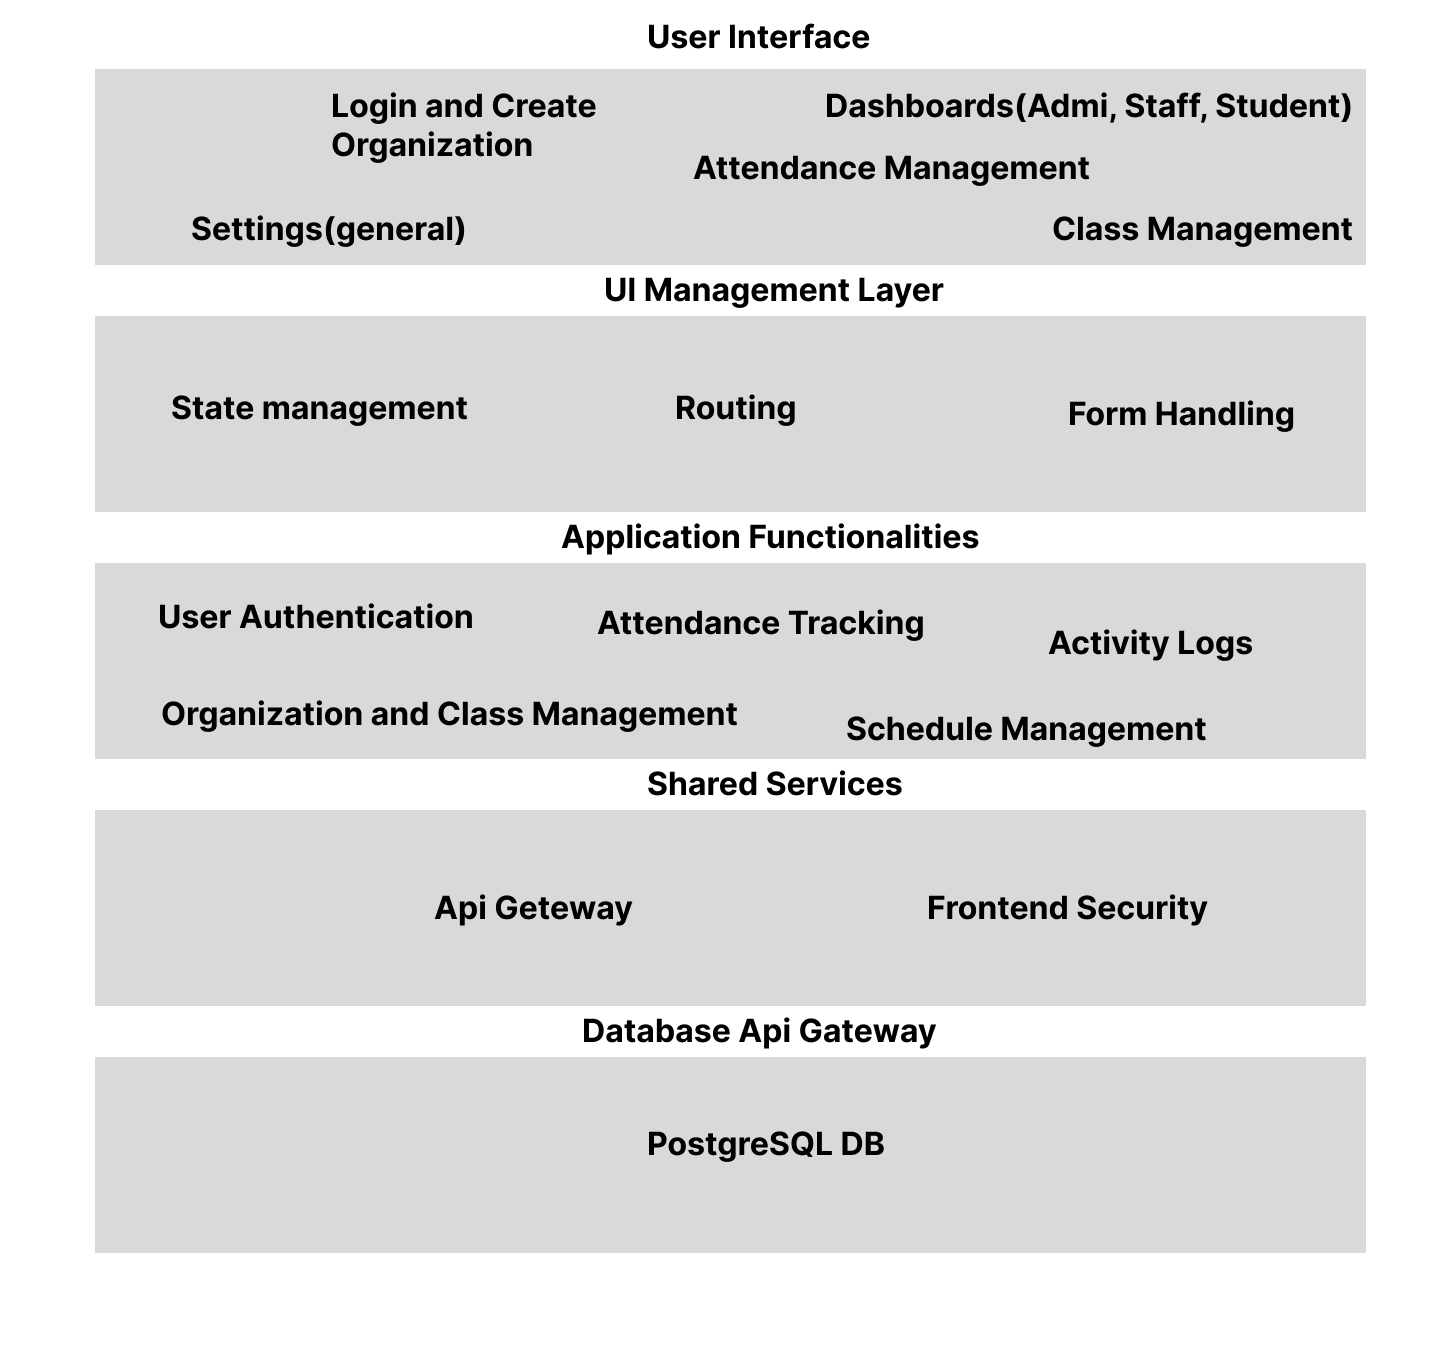
\includegraphics[width=0.8\textwidth]{Arch(frontend.png}
    \caption*{\flushleft Smart Attendance System Architecture Model}
\end{figure}
\end{document}
